\begin{figure}[!t]
\centering
%% ── Left panel ──────────────────────────────────────────────────────────────
\begin{minipage}[t]{0.44\columnwidth}
\centering
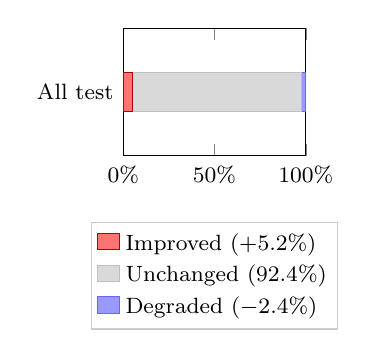
\begin{tikzpicture}
\begin{axis}[
  xbar stacked,
  bar width=14pt,
  width=3.9cm, height=3.2cm,
  xmin=0, xmax=100,
  xtick={0,50,100},
  xticklabel={\pgfmathprintnumber{\tick}\%},
  xticklabel style={font=\footnotesize},
  ytick={0},
  yticklabels={All test},
  yticklabel style={font=\footnotesize},
  ymin=-0.5, ymax=0.5,
  legend style={font=\footnotesize, at={(0.5,-0.52)}, anchor=north,
    legend columns=1, inner sep=2pt, draw=gray!40},
  legend cell align=left,
]
\addplot[fill=red!55, draw=red!70!black]
  coordinates {(5.17, 0)};
\addlegendentry{Improved ($+$5.2\%)}
\addplot[fill=gray!30, draw=gray!50]
  coordinates {(92.43, 0)};
\addlegendentry{Unchanged (92.4\%)}
\addplot[fill=blue!40, draw=blue!60]
  coordinates {(2.44, 0)};
\addlegendentry{Degraded ($-$2.4\%)}
\end{axis}
\end{tikzpicture}
\vspace{2pt}\\
{\footnotesize (a) Per-sample $\Delta$Ord.Prec}
\end{minipage}%
\hfill
%% ── Right panel ─────────────────────────────────────────────────────────────
\begin{minipage}[t]{0.52\columnwidth}
\centering
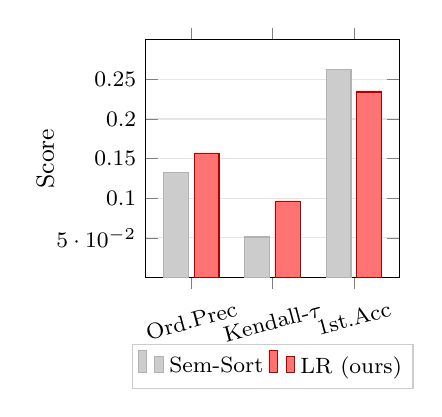
\begin{tikzpicture}
\begin{axis}[
  ybar,
  bar width=9pt,
  width=4.8cm, height=4.6cm,
  symbolic x coords={OrdPrec, KendallTau, FirstAcc},
  xtick=data,
  xticklabels={Ord.Prec, Kendall-$\tau$, 1st.Acc},
  xticklabel style={font=\footnotesize, rotate=15},
  ymin=0.0, ymax=0.30,
  ytick={0.05,0.10,0.15,0.20,0.25},
  scaled y ticks=false,
  yticklabel style={font=\footnotesize},
  ylabel={Score},
  ylabel style={font=\small, yshift=-6pt},
  legend style={font=\footnotesize, at={(0.5,-0.28)}, anchor=north,
    legend columns=2, inner sep=2pt, draw=gray!40},
  legend cell align=left,
  ymajorgrids=true,
  grid style={gray!20, line width=0.4pt},
  enlarge x limits=0.28,
]
\addplot[fill=gray!40, draw=gray!60]
  coordinates {
    (OrdPrec,    0.133)
    (KendallTau, 0.051)
    (FirstAcc,   0.262)
  };
\addlegendentry{Sem-Sort}
\addplot[fill=red!55, draw=red!70!black]
  coordinates {
    (OrdPrec,    0.156)
    (KendallTau, 0.096)
    (FirstAcc,   0.234)
  };
\addlegendentry{LR (ours)}
\end{axis}
\end{tikzpicture}
\vspace{2pt}\\
{\footnotesize (b) Ordering vs.\ 1st.Acc trade-off}
\end{minipage}
\caption{Error analysis of GS-Hybrid+LR vs.\ GS-Hybrid+Sem-Sort on ToolBench.
(a)~92\% of instances are unaffected; LR improves 515 instances ($+$5.2\%) and
degrades 243 ($-$2.4\%). Improved cases share high SkillGraph transition
asymmetry; degraded cases are predominantly single-tool sequences where
pairwise signal is uninformative.
(b)~LR improves global ordering (Ord.Prec $+17\%$; Kendall-$\tau$ $+88\%$) at
a small cost to first-tool accuracy ($-$2.8\,pp), a known property of pairwise
ranking objectives that optimise aggregate agreement rather than position~1.}
\label{fig:error_analysis}
\end{figure}
